% ju 16-Dez-22
\documentclass[a4paper,12pt,fleqn,parskip=half]{scrartcl}
\usepackage[ngerman]{babel}
\usepackage[utf8]{inputenc}
\usepackage[T1]{fontenc}

% Schrift
%\usepackage{lmodern}
\usepackage[osf,sc]{mathpazo} 
\usepackage[scale=.9,semibold]{sourcecodepro}   
\usepackage[osf]{sourcesanspro}  

\usepackage[headsepline]{scrlayer-scrpage}
\pagestyle{scrheadings}
\clearpairofpagestyles

\usepackage[table,dvipsnames,usenames]{xcolor}
\usepackage{textcase}
\usepackage{nameref}
\usepackage{hyperref}
\usepackage{tabularx}
\usepackage{multirow}
\usepackage{multicol}
\usepackage{caption, booktabs}
\usepackage{graphicx} 
\usepackage{scrhack}    
\usepackage{url}%% Links
\usepackage[inline]{enumitem}
\usepackage{pifont}
\usepackage{eurosym}% \euro 20,-
\usepackage{amsmath}
\usepackage{amsfonts}
\usepackage{amssymb}
\usepackage{array}            % Extending the array and tabular environments
\usepackage{chngcntr}         % Change the resetting of counters
\usepackage[version=4]{mhchem}
\usepackage{stmaryrd}
\usepackage{siunitx}
\usepackage{float}
\usepackage{csquotes}
\usepackage{subcaption}
\usepackage{mathtools}
\usepackage{icomma}%Dezimaltrennzeichen
\usepackage{multimedia}%Video: \movie[externalviewer]{(video.mov)}{video.mov}
\usepackage{epstopdf}
\usepackage{footnote}
\usepackage{qrcode}% Anwendung: \qrcode[hyperlink,level=Q,version=2,height=1cm]{\website}
\usepackage{underscore}% Unterstrich ____

% PDF Dokumente einbinden
\usepackage{pdfpages}% \includepdf[pages=-]{Tabellen/Excel.pdf}
\RequirePackage{lastpage}  % Pagecounter

\addto\captionsngerman{%
\renewcommand{\figurename}{Abb.}
\renewcommand{\tablename}{Tab.}
}

% listings
\usepackage{listings}
\lstset{basicstyle=\linespread{1}\ttfamily\small,floatplacement=!htb,captionpos=t,abovecaptionskip=.5\baselineskip,belowcaptionskip=.5\baselineskip,upquote=true,showstringspaces=false,inputencoding=utf8,tabsize=4,
    	keywordstyle=\bfseries ,
	commentstyle=\color{rot5},
	stringstyle=\color{orange},
	breaklines=true,
  	postbreak=\mbox{\textcolor{black}{$\hookrightarrow$}\space},
	breakatwhitespace=false
}
\lstset{literate={á}{{\'a}}1 {é}{{\'e}}1 {í}{{\'i}}1 {ó}{{\'o}}1 {ú}{{\'u}}1 {Á}{{\'A}}1 {É}{{\'E}}1 {Í}{{\'I}}1 {Ó}{{\'O}}1 {Ú}{{\'U}}1 {à}{{\`a}}1 {è}{{\`e}}1 {ì}{{\`i}}1 {ò}{{\`o}}1 {ù}{{\`u}}1 {À}{{\`A}}1 {È}{{\'E}}1 {Ì}{{\`I}}1 {Ò}{{\`O}}1 {Ù}{{\`U}}1 {ä}{{\"a}}1 {ë}{{\"e}}1 {ï}{{\"i}}1 {ö}{{\"o}}1 {ü}{{\"u}}1 {Ä}{{\"A}}1 {Ë}{{\"E}}1 {Ï}{{\"I}}1 {Ö}{{\"O}}1 {Ü}{{\"U}}1 {â}{{\^a}}1 {ê}{{\^e}}1 {î}{{\^i}}1 {ô}{{\^o}}1 {û}{{\^u}}1 {Â}{{\^A}}1 {Ê}{{\^E}}1 {Î}{{\^I}}1 {Ô}{{\^O}}1 {Û}{{\^U}}1 {œ}{{\oe}}1 {Œ}{{\OE}}1 {æ}{{\ae}}1 {Æ}{{\AE}}1 {ß}{{\ss}}1 {ű}{{\H{u}}}1 {Ű}{{\H{U}}}1 {ő}{{\H{o}}}1 {Ő}{{\H{O}}}1 {ç}{{\c c}}1 {Ç}{{\c C}}1 {ø}{{\o}}1 {å}{{\r a}}1 {Å}{{\r A}}1 {€}{{\EUR}}1 {£}{{\pounds}}1 {~}{{\textasciitilde}}1 {-}{{-}}1 }

% bibliography
\usepackage[
    bibencoding=utf8,
    backend=biber,% bibtex, biber
    backref=false,backrefstyle=three+,url=true,urldate=comp,abbreviate=false,maxnames=20
]{biblatex} %Paket laden
\DeclareBibliographyCategory{cited}
\let\defaultcite\cite\renewcommand*\cite[2][]{\addtocategory{cited}{#2}\defaultcite[#1]{#2}}
\let\defaulttextcite\textcite\renewcommand*\textcite[2][]{\addtocategory{cited}{#2}\defaulttextcite[#1]{#2}}
\setcounter{biburllcpenalty}{7000}
\setcounter{biburlucpenalty}{8000}
\AfterPackage{biblatex}{
	\PreventPackageFromLoading[\errmessage{Sie haben versucht, das Cite-Paket zu laden, das nicht mit biblatex kompatibel ist.}]{cite}
}

\hypersetup{%
	%pdftitle={\titel},
	%pdfsubject={Latex},
	%pdfauthor={\autor},
	%pdfcreator={\autor}, 
	bookmarksnumbered=true,
	breaklinks=true,
	%colorlinks=true,	   
	linkcolor=rot5,		
	filecolor=blau5,		
	urlcolor=blau5,			
	citecolor=ForestGreen
}

\linespread{1.1}
\setlist{itemsep=0pt}
\widowpenalty10000
\clubpenalty10000
\tolerance1000   

\usepackage[left=2cm,right=2cm,top=1cm,bottom=1cm,includeheadfoot]{geometry}
%\usepackage[left=4cm,right=2cm,top=1cm, bottom=1cm,includeheadfoot]{geometry}
%\usepackage[left=6cm,right=1cm,top=1cm, bottom=1cm,includeheadfoot]{geometry}
%\usepackage[landscape=true,left=2cm,right=2cm,top=1cm,bottom=1cm,includeheadfoot]{geometry}%quer

% eigene Farbe definieren
% Adobe Prozessfarben: CMYK: 100,50,0,35 -> 1,0.5,0,0.35
\definecolor{orange}{cmyk}{0,0.55,0.61,0}   % 0,55,61,0
\definecolor{blau5}{cmyk}{1,0.77,0.1,0.01}  % 100,77,10,
\definecolor{rot5}{cmyk}{0.22,1,1,0.19}     % 22,100,100,19
\definecolor{grau2}{cmyk}{0,0,0,0.1}        % 0,0,0,40
\definecolor{blau}{cmyk}{0.93,0.66,0,0.21}% 

% Literatur
\bibliography{content/literatur}
\bibliography{content/literatur-kfz}
\bibliography{content/literatur-sport}

%%%%%%%%%%%%%%%%%%%%%%%%%%%%%%%%%%%%%%%%%%%%%%%%%%%%%%%
\newcommand{\name}{Jan Unger}
\newcommand{\thema}{04-Generator}
\newcommand{\quelle}{\name}
\newcommand{\website}{https://bw-ju.de/}
\newcommand{\github}{https://github.com/ju1-eu}
%%%%%%%%%%%%%%%%%%%%%%%%%%%%%%%%%%%%%%%%%%%%%%%%%%%%%%%

\ihead{\textbf{Quelle:} \quelle}%{Kopfzeile innen}
\ohead{\textbf{Datum:} \today}  %{Kopfzeile außen}
\ifoot{\textbf{Thema:} \thema}  %{Fußzeile  innen}
\ofoot{Seite {\thepage} von {\pageref{LastPage}}}%{Fußzeile  außen}

\title{\thema}
\author{\name}
\date{\today}

\begin{document}
	%%%%%%%%%%%%%%%%%%%%%%%%%%%%%%%%%%%%%%%%%%%%%%%%%%%%%%%%%%%%%%%%%%
	\begin{abstract}
		\center
		\textbf{\Large \thema}%14pt
		
		\vspace{1.5em}
		%\datum	
		%\qrcode[hyperlink,level=Q,version=2,height=1cm]{\website}
		\qrcode[hyperlink,level=Q,version=2,height=1cm]{\github}
		
		\vspace{1.5em} 
		\raggedright
		\textbf{\large Keywords}
		% Checkliste
		\begin{itemize}[label=\checkmark]
			\item Begriff
		\end{itemize}
	\end{abstract}
    %%%%%%%%%%%%%%%%%%%%%%%%%%%%%%%%%%%%%%%%%%%%%%%%%%%%%%%%%%%%%%%%%%

	% anpassen
	%\input{content/tex/neu}
	%ju 16-Dez-22 04-Generator.tex
\textbf{Drehstromgenerator / Lichtmaschine / Generator}

Quelle: Fabian Lindenberg, Kfz-Technik einfach erklärt \footnote{\url{https://www.youtube.com/watch?v=O7ydsAZ6bes}}

\section{Komponenten}\label{komponenten}

\begin{enumerate}
\item
  \textbf{Regler} (Multifunktionsregler hat keine Erregendioden, bekommt
  Spg. von Kl.30)
\item
  \textbf{Schleifringe}
\item
  \textbf{Gleichrichterdioden} (Leistungsdioden)
\item
  \textbf{Klauenpolläufer} (mit Riemenscheibe $\to$ Antrieb Motor und
  Schleifringe $\to$ Regler)
\item
  \textbf{Erregerwicklung} (Rotor, dreht sich, sitzt im Klauenpolläufer)
\item
  \textbf{Ständerwicklung} (mit Gehäuse, Stator, steht)
\item
  \textbf{Lüfter}
\end{enumerate}

\textbf{Diodenplatte:} 6x Gleichrichterdioden (3x Plusdioden, 3x
Minusdioden), 3x Erregerdioden

\textbf{Klauenpolläufer} 12 Pole (je 6 Nord- und Südpole) x 3
Statorspulen = 36 Halbwellen = 1x Umdrehung. Batterie und Kondensator
glättet die Gleichspannung.

\begin{figure}[!ht]% hier: !ht
\centering
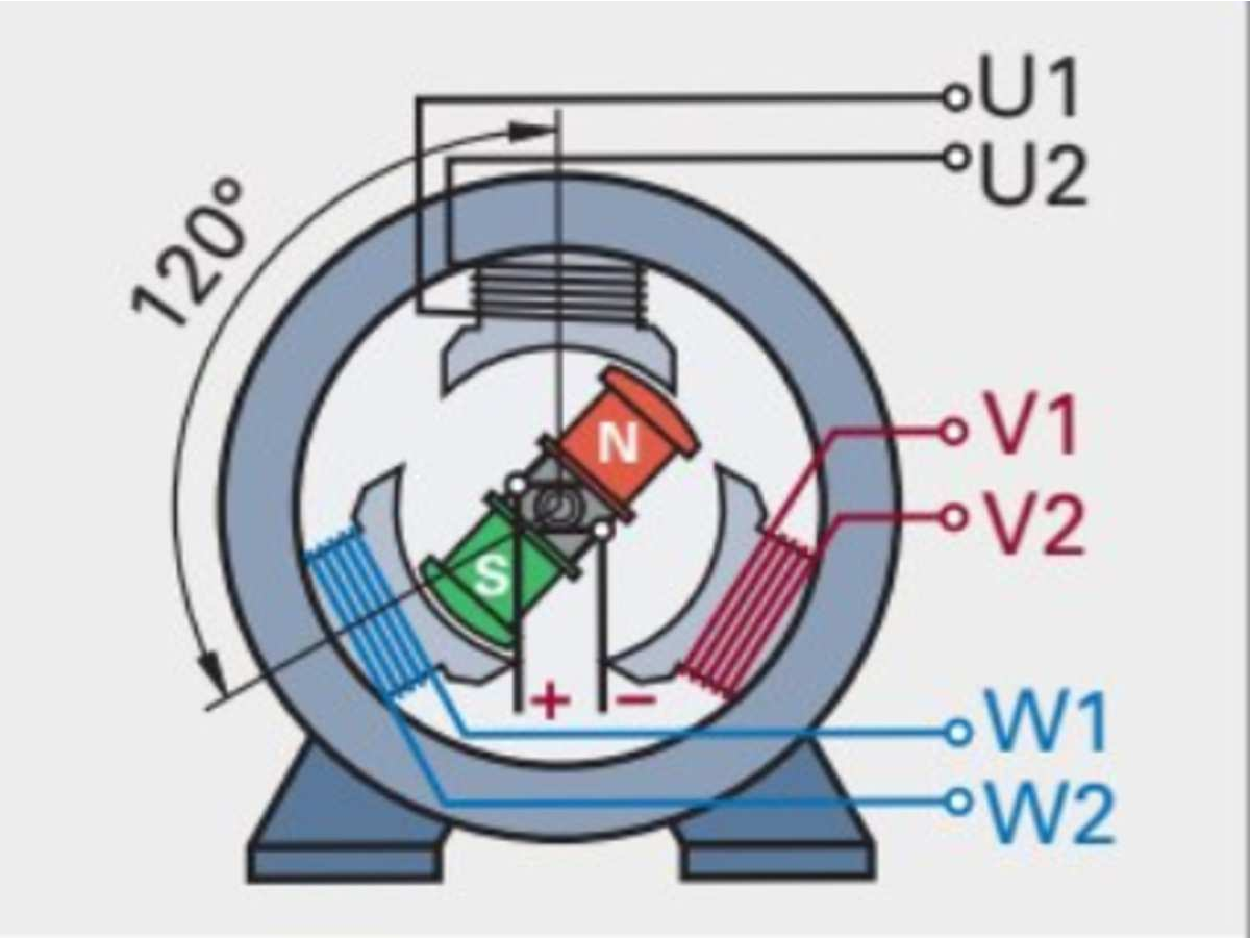
\includegraphics[width=0.4\textwidth]{images/Generator/Generator-11.pdf}
\caption{Generatoraufbau - Drei Ständerwicklungen U,V,W und ein Polrad}
%\label{fig:}%% anpassen
\end{figure}

\begin{figure}[!ht]% hier: !ht
\centering
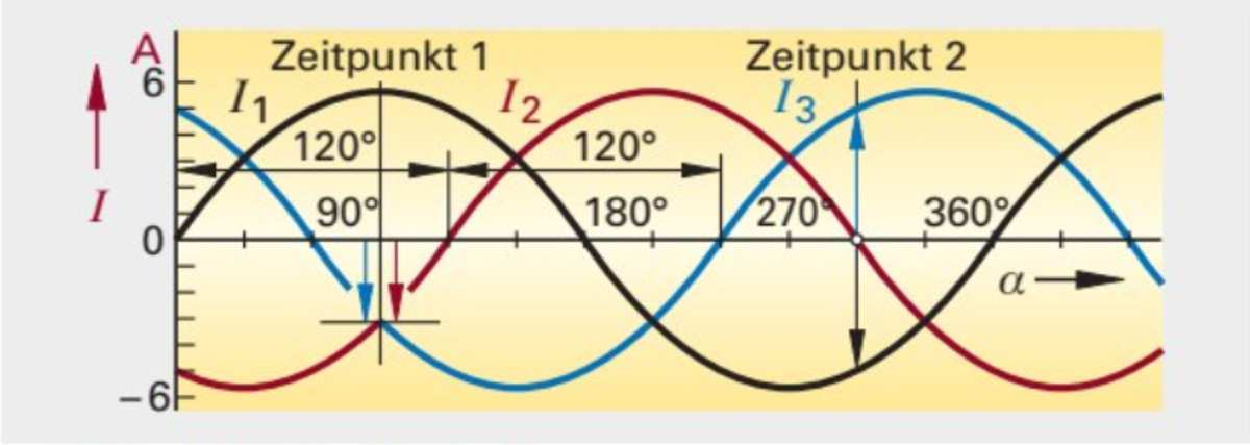
\includegraphics[width=0.4\textwidth]{images/Generator/Generator-8.pdf}
\caption{3 Wechselspannungen mit 120° Phasenverschiebung}
%\label{fig:}%% anpassen
\end{figure}

\section{Multifunktionsregler}\label{multifunktionsregler}

\begin{figure}[!ht]% hier: !ht
\centering
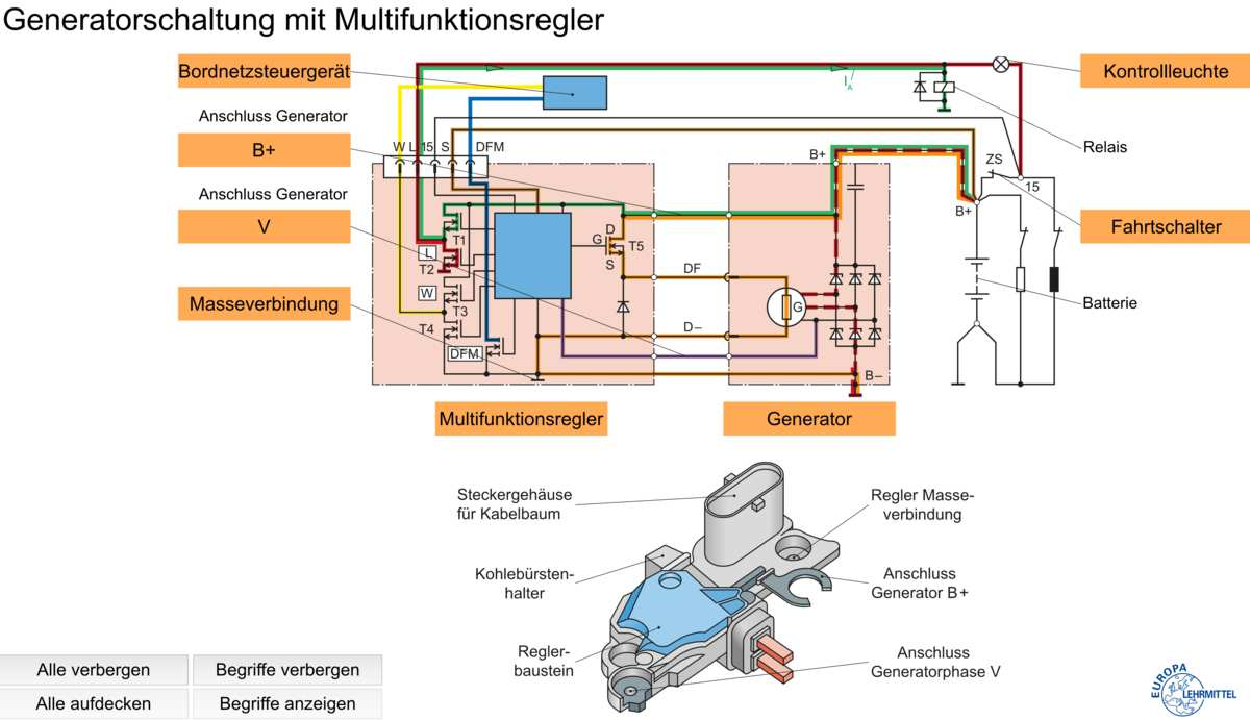
\includegraphics[width=0.85\textwidth]{images/Generator/Generator-1.pdf}
\caption{Schaltung Generator mit Multifunktionsregler, Quelle:
Europa-Verlag}
%\label{fig:}%% anpassen
\end{figure}

\textbf{Merkmale}

\begin{enumerate}
\item
  Unterstützung Motormanagement
\item
  Batterieüberwachung
\item
  Auslastungsüberwachung
\item
  Temperaturabhängige Ladespannung
\item
  Schutz gegen Überlastung / Kurzschluss
\item
  Interne Fehlerdiagnose $\to$ SG
\item
  Vorerregerstrom Steuern (Dreht sich der Generator)
\item
  Low-Response (Start \& Fahrt: Belastung des Generators wird verzögert
  zugeschaltet, Kraftstoff sparen)
\end{enumerate}

\newpage

\section{Generator prüfen}\label{generator-pruefen}

\textbf{Ladekontrolle an}

\begin{itemize}
\item
  Zündung an, Motor steht
\item
  Erregungsunterbrechung
\item
  Überspannung
\item
  Keilriemen gerissen
\item
  Leitungsunterbrechung
\item
  Defekte Masseverbindung
\end{itemize}

\textbf{Generator Anschluss}

\begin{enumerate}
\item
  \textbf{W} Drehzahl
\item
  \textbf{B-} Masse
\item
  \textbf{D+} Ladekontrolle, Erregerwicklung
\item
  \textbf{B+} Batterie
\item
  \textbf{DF} Regler, Erregerwicklung
\end{enumerate}

\textbf{Generator mit Multifunktionsregler Anschluss}

\begin{enumerate}
\item
  \textbf{L} Ladekontrollleuchte
\item
  \textbf{S} Sense, Batterie überwachen
\item
  \textbf{W} Drehzahlsignal zur Regelung des Vorerregerstroms
\item
  \textbf{V} Phasenspannung überwachen (Fehlerdiagnose, Beispiel: def.
  Keilriemen erkennen)
\item
  \textbf{DFM} PWM-Signal des Erregerstroms zur Auslastung des
  Generators
\end{enumerate}

\textbf{Erregerspannung und Generatorspannung / Ladespannung messen}

\begin{itemize}
\item
  Unter Belastung (Verbraucher EIN)
\item
  Motordrehzahl (ca. 1800 - 2200 1/min)
\item
  \textbf{Erregerspannung}

  \begin{itemize}
  \item
    Messpunkt: (D+ und D-/B-/Masse)
  \end{itemize}
\item
  \textbf{Generatorspannung / Ladespannung}

  \begin{itemize}
  \item
    Messpunkt: (B+ und D-/B-/Masse)
  \end{itemize}
\end{itemize}

\textbf{Fehler}

\begin{enumerate}
\item
  Oberwelle normal
\item
  Minusseitig eine Sperrdiode defekt $\to$ Eine Welle wäre weg,
  Leistung von der Spule fehlt
\item
  Erregerdiode defekt $\to$ Ladespannung geht runter
\end{enumerate}

\begin{figure}[!ht]% hier: !ht
\centering
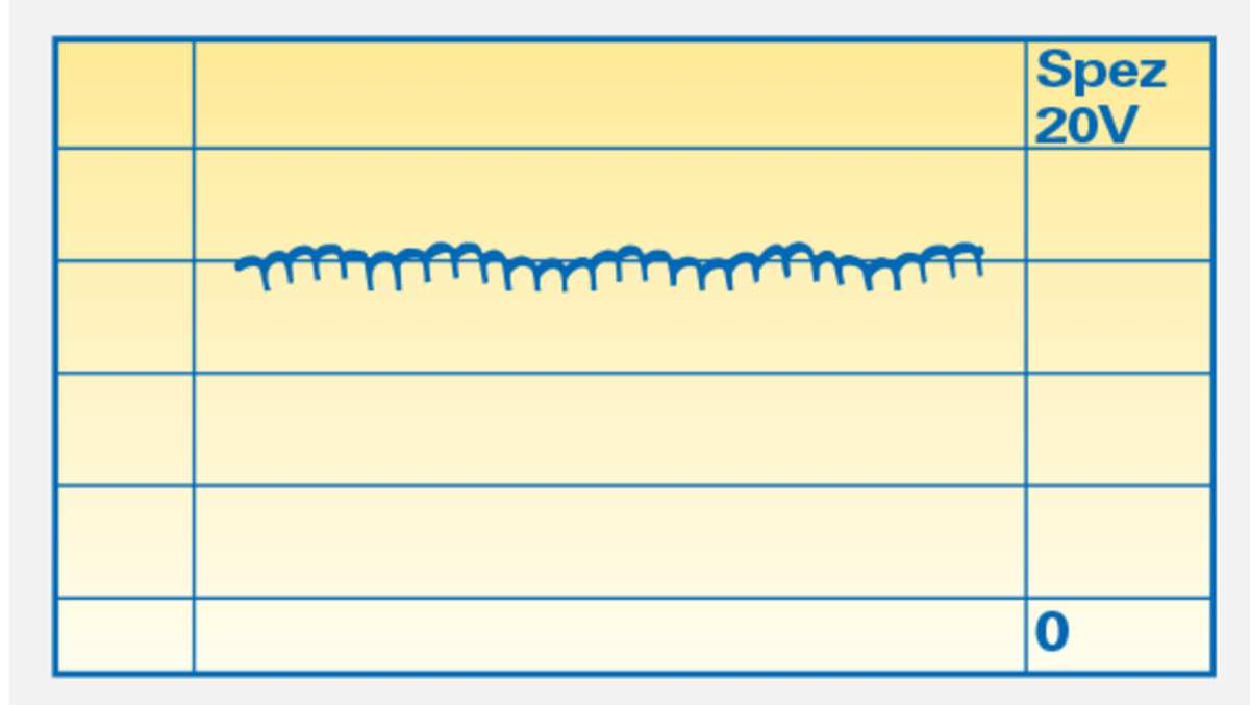
\includegraphics[width=0.4\textwidth]{images/Generator/Generator-2.pdf}
\caption{Generator Gutbild, Quelle: Europa-Verlag}
%\label{fig:}%% anpassen
\end{figure}

\begin{figure}[!ht]% hier: !ht
\centering
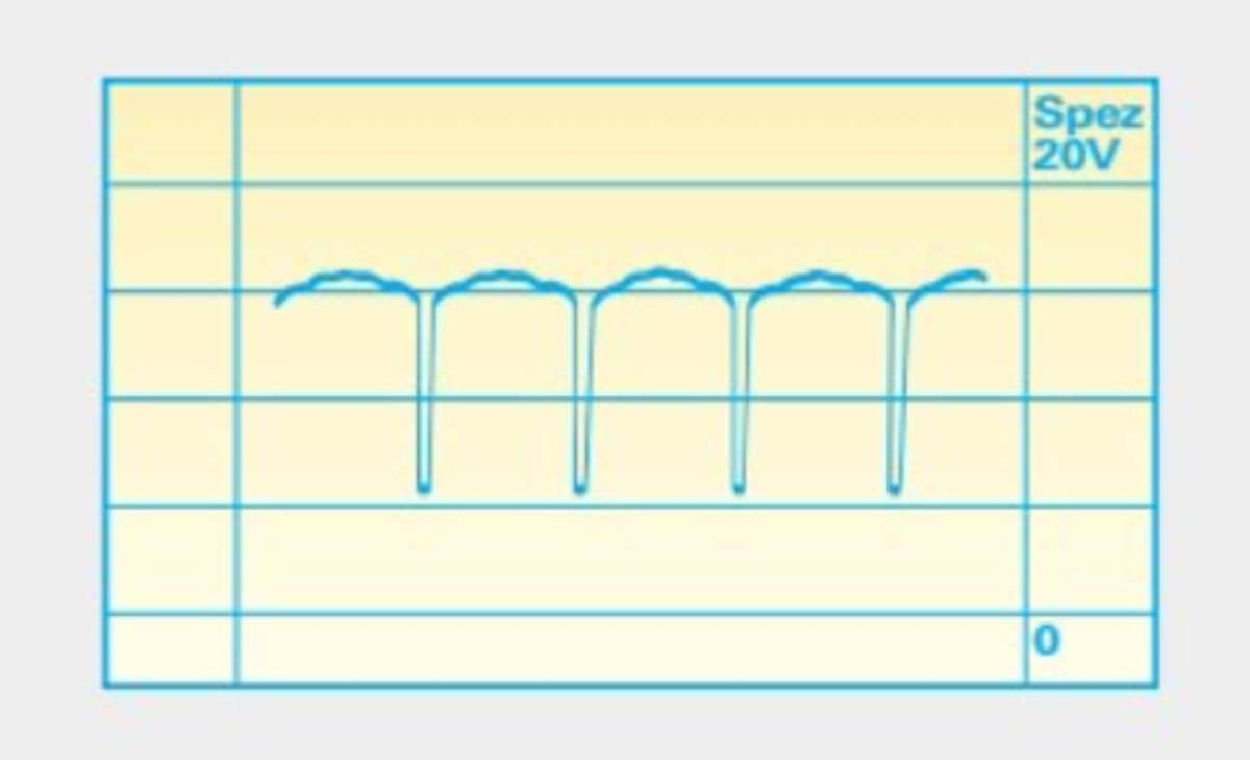
\includegraphics[width=0.4\textwidth]{images/Generator/Generator-5.pdf}
\caption{Generator Fehler - Unterbrechung einer Minusdiode, Quelle:
Europa-Verlag}
%\label{fig:}%% anpassen
\end{figure}

\newpage

\section{Energieumwandlung}\label{energieumwandlung}

kinetische Energie + elektrische Energie (Drehmoment) $\to$
\textbf{Generator} $\to$ elektrische Energie

\textbf{Induktion} mit ein Magnetfeld Elektronen bewegen.

Magnet (Nordpol/Südpol, anziehen / abstoßen)

Rechte-Handregel: Magnetfeld bestimmen

\begin{enumerate}
\item
  Stromdurchflossener Leiter $\to$ erzeugt Magnetfeld
\item
  Stromdurchflosse Spule $\to$ erzeugt großes Magnetfeld
\item
  Rotor (Erregerwicklung, Fremderregt) und Stator (mit 3x Spulen, U / V
  / W) $\to$ erzeugt drehbares Magnetfeld
\end{enumerate}

\textbf{indizierte Spannung} ist abhängig

\begin{enumerate}
\item
  Anzahl Wicklungen von Statorspulen
\item
  Drehzahl Generator
\item
  Stärke des Magnetfeldes
\item
  Fläche
\end{enumerate}

\begin{figure}[!ht]% hier: !ht
\centering
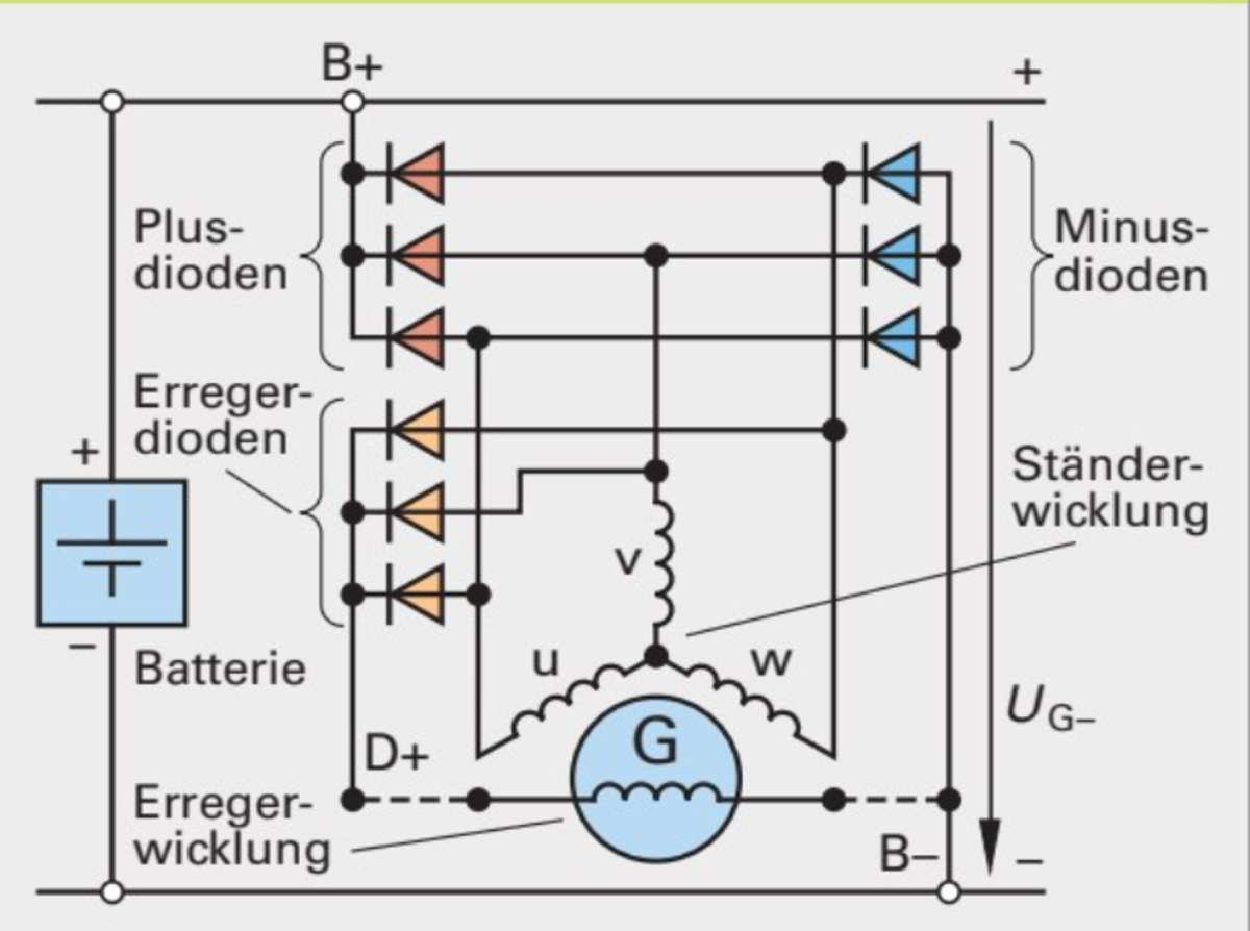
\includegraphics[width=0.3\textwidth]{images/Generator/Generator-6.pdf}
\caption{Drehstrom - Brückenschaltung}
%\label{fig:}%% anpassen
\end{figure}

\begin{figure}[!ht]% hier: !ht
\centering
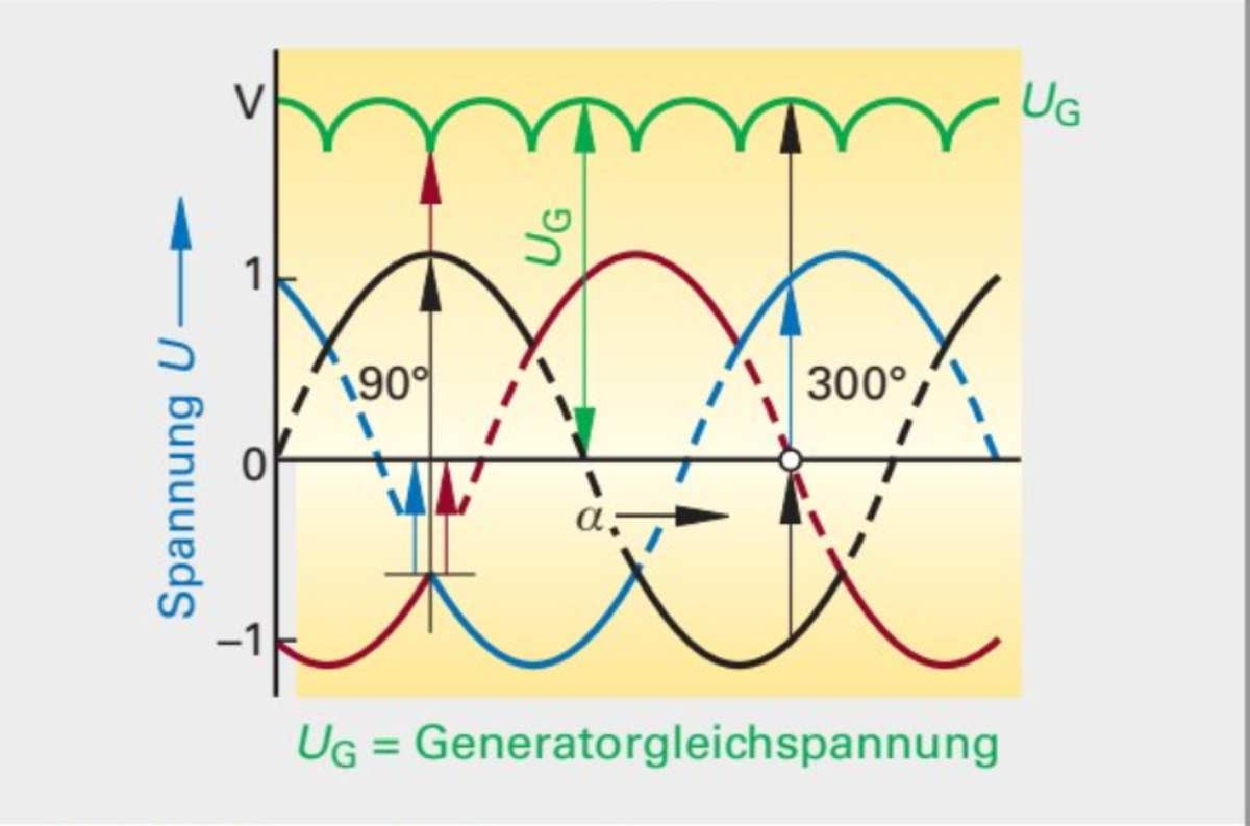
\includegraphics[width=0.3\textwidth]{images/Generator/Generator-7.pdf}
\caption{Gleichrichtung der Generatorspannung}
%\label{fig:}%% anpassen
\end{figure}

\newpage

\section{Energiefluss}\label{energiefluss}

\begin{figure}[!ht]% hier: !ht
\centering
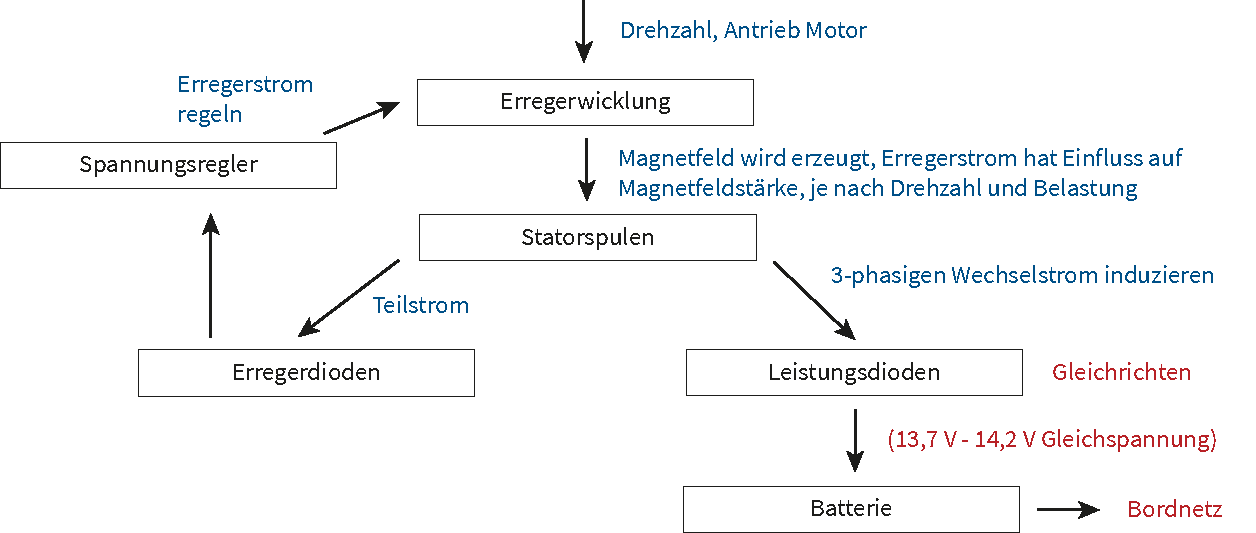
\includegraphics[width=0.8\textwidth]{images/Generator/Generator-Energiefluss.pdf}
\caption{Energiefluss}
%\label{fig:}%% anpassen
\end{figure}

\textbf{Erregerwicklung} sitzt im Klauenpolläufer, erzeugt Magnetfeld
welches auf die Statorspulen wirkt

\textbf{Statorspulen} Sternschaltung, Durch das Magnetfeld der
Erregerwicklung wird eine Spannung induziert. 3x Spulen um 120° versetzt
$\to$ 3-phasige Wechselspannung

\textbf{Leistungsdioden} Richten die 3-phasige Wechselspannung in eine
Gleichspannung um.

\textbf{Erregerdioden} Spannungsversorgung des Spannungsreglers.

\textbf{Spannungsregler} regelt den Erregerstrom und variiert damit die
Stärke des Magnetfeldes. \textbf{Ladespannung ist Konst.} bei allen
Motordrehzahlen (Leerlauf - Vollast) u. Belastungen (Verbraucher).
\textbf{Wie?} Je stärker das Magnetfeld, desto größer ist die Spannung
die in den Statorspulen induziert wird.

\newpage

\section{Schaltung}\label{schaltung}

\begin{figure}[!ht]% hier: !ht
\centering
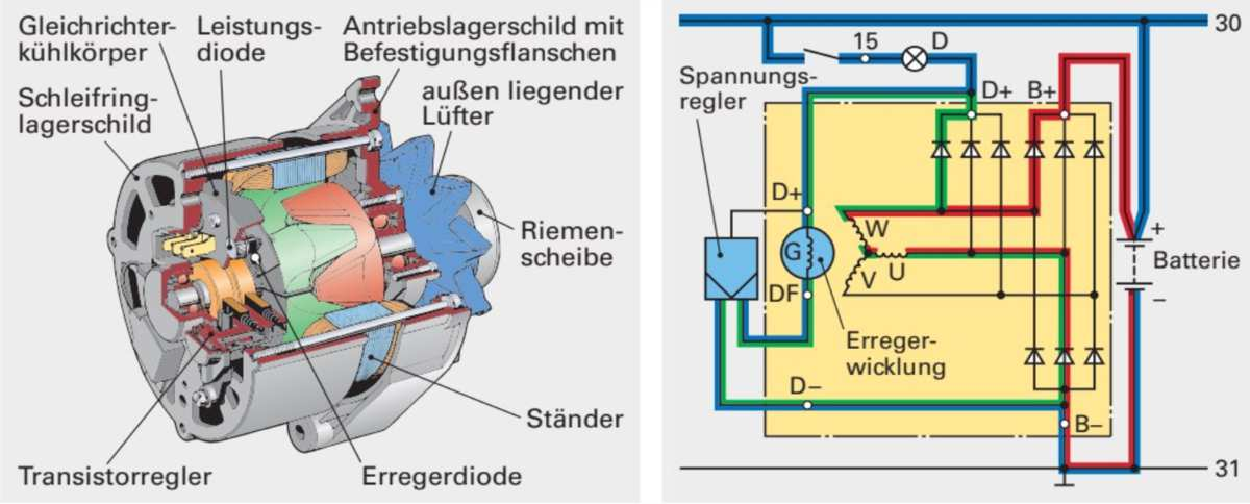
\includegraphics[width=0.85\textwidth]{images/Generator/Generator-9.pdf}
\caption{Schaltung Generator mit Transistorregler, Quelle:
Europa-Verlag}
%\label{fig:}%% anpassen
\end{figure}

Zündung an, Motor steht

\textbf{Vorerregerstromkreis (blau)} B+ $\to$ Fahrtschalter $\to$
Ladekontrolllampe $\to$ D+ $\to$ Erregerwicklung $\to$ Regler DF
$\to$ Masse $\to$ B-

Zündung an, Motor läuft

\textbf{Erregerstromkreis (grün)} Ständerwicklung $\to$ Erregerdioden
$\to$ D+ $\to$ Erregerwicklung $\to$ Regler DF $\to$ Regler D-
$\to$ Minusdioden $\to$ Ständerwicklung

\textbf{Ladestromkreis (rot)} Ständerwicklung $\to$ Plusdioden $\to$
B+ $\to$ Verbraucher $\to$ Masse $\to$ Minusdioden $\to$
Ständerwicklung

\newpage

\begin{figure}[!ht]% hier: !ht
\centering
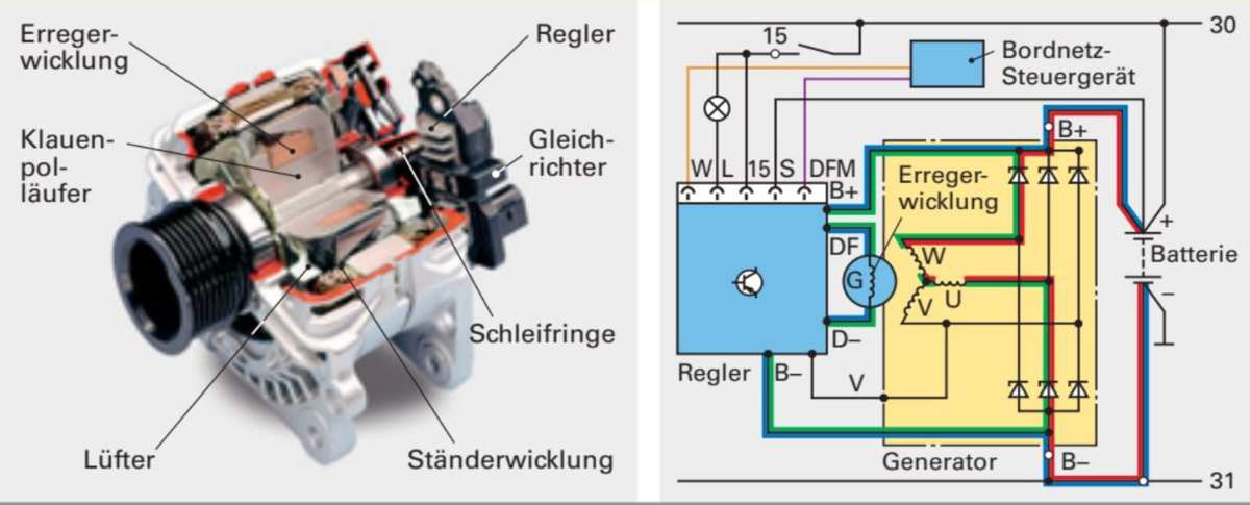
\includegraphics[width=0.85\textwidth]{images/Generator/Generator-10.pdf}
\caption{Schaltung Generator mit Multifunktionsregler, Quelle:
Europa-Verlag}
%\label{fig:}%% anpassen
\end{figure}

\textbf{Vorerregerstromkreis (blau)} B+ $\to$ Erregerwicklung $\to$
Regler DF $\to$ Reglerendstufe $\to$ B-

Zündung an, Motor läuft

\textbf{Erregerstromkreis (grün)} Ständerwicklung $\to$ Plusdioden
$\to$ Regler B+ $\to$ Regler DF $\to$ Erregerwicklung $\to$
Regler D- $\to$ Regler B- $\to$ Minusdioden $\to$ Ständerwicklung

\textbf{Ladestromkreis (rot)} Ständerwicklung $\to$ Plusdioden $\to$
B+ $\to$ Verbraucher $\to$ Masse $\to$ Minusdioden $\to$
Ständerwicklung


	%%%%%%%%%%%%%%%%%%%%%%%%%%%%%%%%%%%%%%%%%%%%%%%%%%%%%%%%%%%%%%%%%%
    % Bibliographie
    \printbibliography[category=cited]
\end{document}
